\section{Introducción}
\justifying

\begin{frame}{Grafeno}
	Es una de las formas alotrópicas del carbono.

	\begin{figure}
		\subfigure[Propiedades del grafeno]{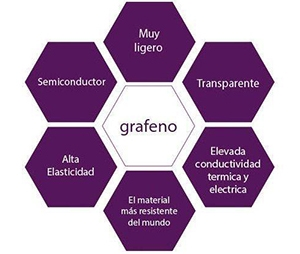
\includegraphics[width=4cm]{graficas/propiedadesGrafeno.jpg}}
		\subfigure[Alótropos del carbono]{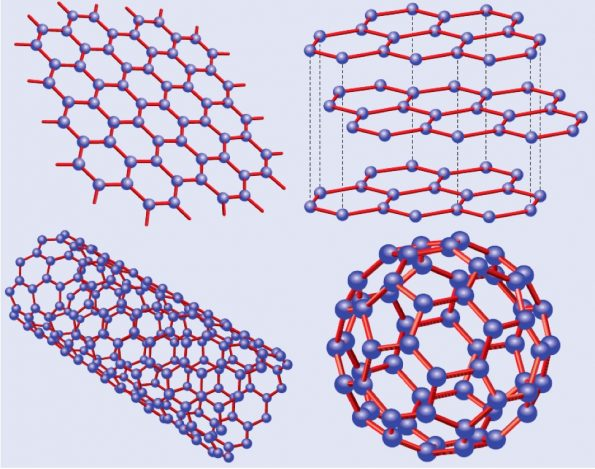
\includegraphics[width=4cm]{graficas/alotropo.jpg}}
		\caption{Grafeno, \textit{Tomado de }\cite{Neto2006} }
	\end{figure}
\end{frame}

\begin{frame}
	Las oscilaciones magnéticas son un fenómeno conocido en la física de la materia condensada, generalmente observado a bajas temperaturas.
	En el grafeno, persiste incluso a temperaturas ambiente. Esto se atribuye a la periodicidad de las superredes de grafeno \cite{Kumar2017}.

	\begin{figure}
		\subfigure[Superred de grafeno]{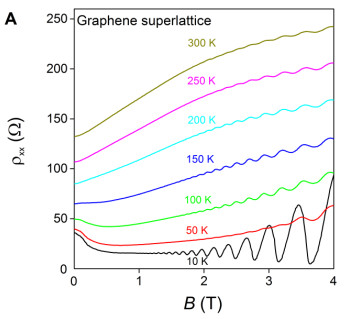
\includegraphics[width=4cm]{graficas/oscilaciones_superred.jpg}}
		\subfigure[grafeno]{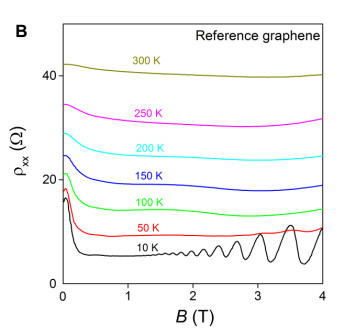
\includegraphics[width=4cm]{graficas/oscilaciones_grafeno.jpg}}
	\caption{$\rho$ vs $B$ a diferentes temperaturas. \textit{Tomadas de \cite{Kumar2017}}}
	\end{figure}
\end{frame}

\begin{frame}
	\begin{multicols}{2}
		Los sistemas electrónicos tambien presentan oscilaciones magnéticas,
		referidos a las mariposas de Hofstadter (HB) \cite{Yu2014}-\cite{Yang2016}.\\
		\vspace{0.5cm}
		Estudios de transporte eléctrico en superredes de grafeno sobre h-BN \cite{Yankowitz2012}
		muestran características de las HB originadas en la superred en un campo magnético \cite{BenShalom2016}.
		\begin{figure}
			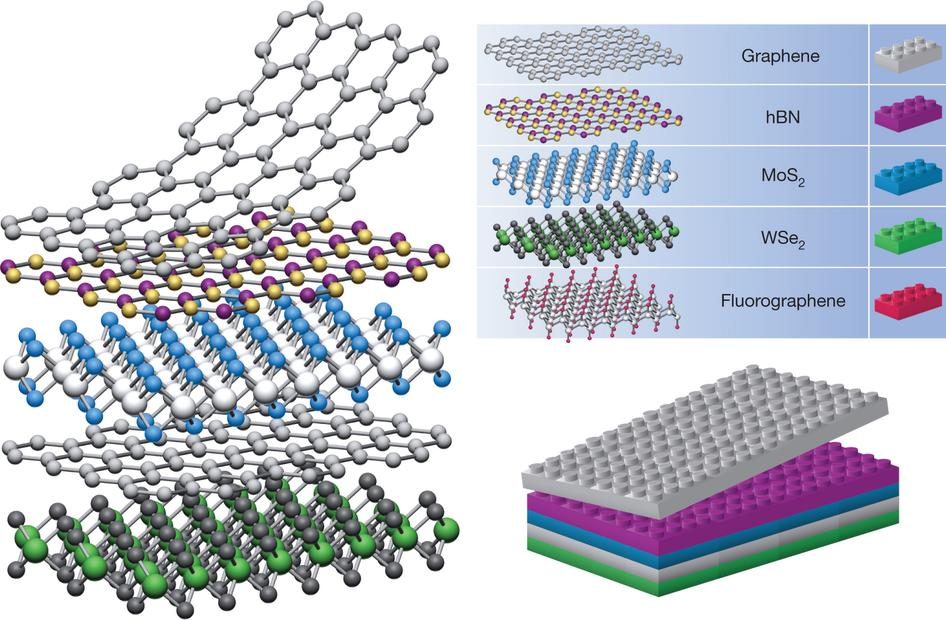
\includegraphics[width=6cm]{graficas/heterostructures.jpg}
			\caption{Superredes de grafeno. \textit{Tomado de} \cite{Geim2013}}
			\label{heterostructures}
		\end{figure}
	\end{multicols}
\end{frame}
